%=========================================================
\chapter{Requerimientos del sistema}	
\label{cap:reqSist}

	Este capítulo describe ...

%---------------------------------------------------------
\section{Requerimientos funcionales}

\cdtInstrucciones{
	Identifique y describa los requerimientos funcionales del sistema señalando: id, nombre, descripción y prioridad.
}


\begin{table}[htbp!]
	\begin{requerimientos}
		\FRitem{RF1}{Registro de vehículos}{El sistema debe permitir el registro, consulta y actualización de los vehículos con los que cuenta la empresa con el fin de hacer una correcta planeación de entregas.}{A}{RU1}
		\FRitem{...}{...}{...}{...}{...}
	\end{requerimientos}
    \caption{Requerimientos funcionales del sistema.}
    {\footnotesize\em Para leer correctamente esta tabla vea la leyenda en la Tabla~\ref{tbl:leyendaRF} en la página~\pageref{tbl:leyendaRF}.}
    \label{tbl:reqFunc}
\end{table}

%---------------------------------------------------------
\section{Requerimientos no funcionales}

\cdtInstrucciones{
	Identifique y escriba los requerimientos no funcionales del sistema. describa como se planea implementar cada uno de ellos.\\
}

\begin{table}[hbtp!]
    \begin{NFRequerimientos}
    	\NFRitem{NF1}{Fiabilidad}{
			% Necesidad
			Que el sistema se ejecute correctamente y libre de defectos
		}{
			% Estrategia
			Se realizarán pruebas exahustivas al menos hasta que el sistema ejecute correctamente todas las funciones de prioridad igual o superior a ``Baja'' con cero defectos.
		}{RU7}
    	\NFRitem{NF2}{...}{
			% Necesidad
			...
		}{
			% Estrategia
			...
		}{...}
    \end{NFRequerimientos}
    \caption{Requerimientos no funcionales del sistema.}
    \label{tbl:reqNF}
\end{table}

%---------------------------------------------------------
\section{Especificación de plataforma}	

\cdtInstrucciones{
	Coloque un diagrama y su descripción para aclarar el tipo de solución propuesta. \\
	
 En esta sección se debe aclarar:
	
\begin{description}
	\item[Tipo de sistema:] Web, aplicación móvil, de escritorio, híbrida, etc.
	\item[Software requerido:] Programas que se deberán instalar, desde el sistema operativo, compiladores, interpretes, servidores, etc.
	\item[Hardware requerido:] CPU, núcleos, velocidad, memoria, disco duro, etc.
	\item[servicios:] De conexión, seguridad, firewall, respaldo de energía, redundancia, uso de raids, etc.
\end{description}
}

\begin{figure}[htbp!]
	\begin{center}
		\fbox{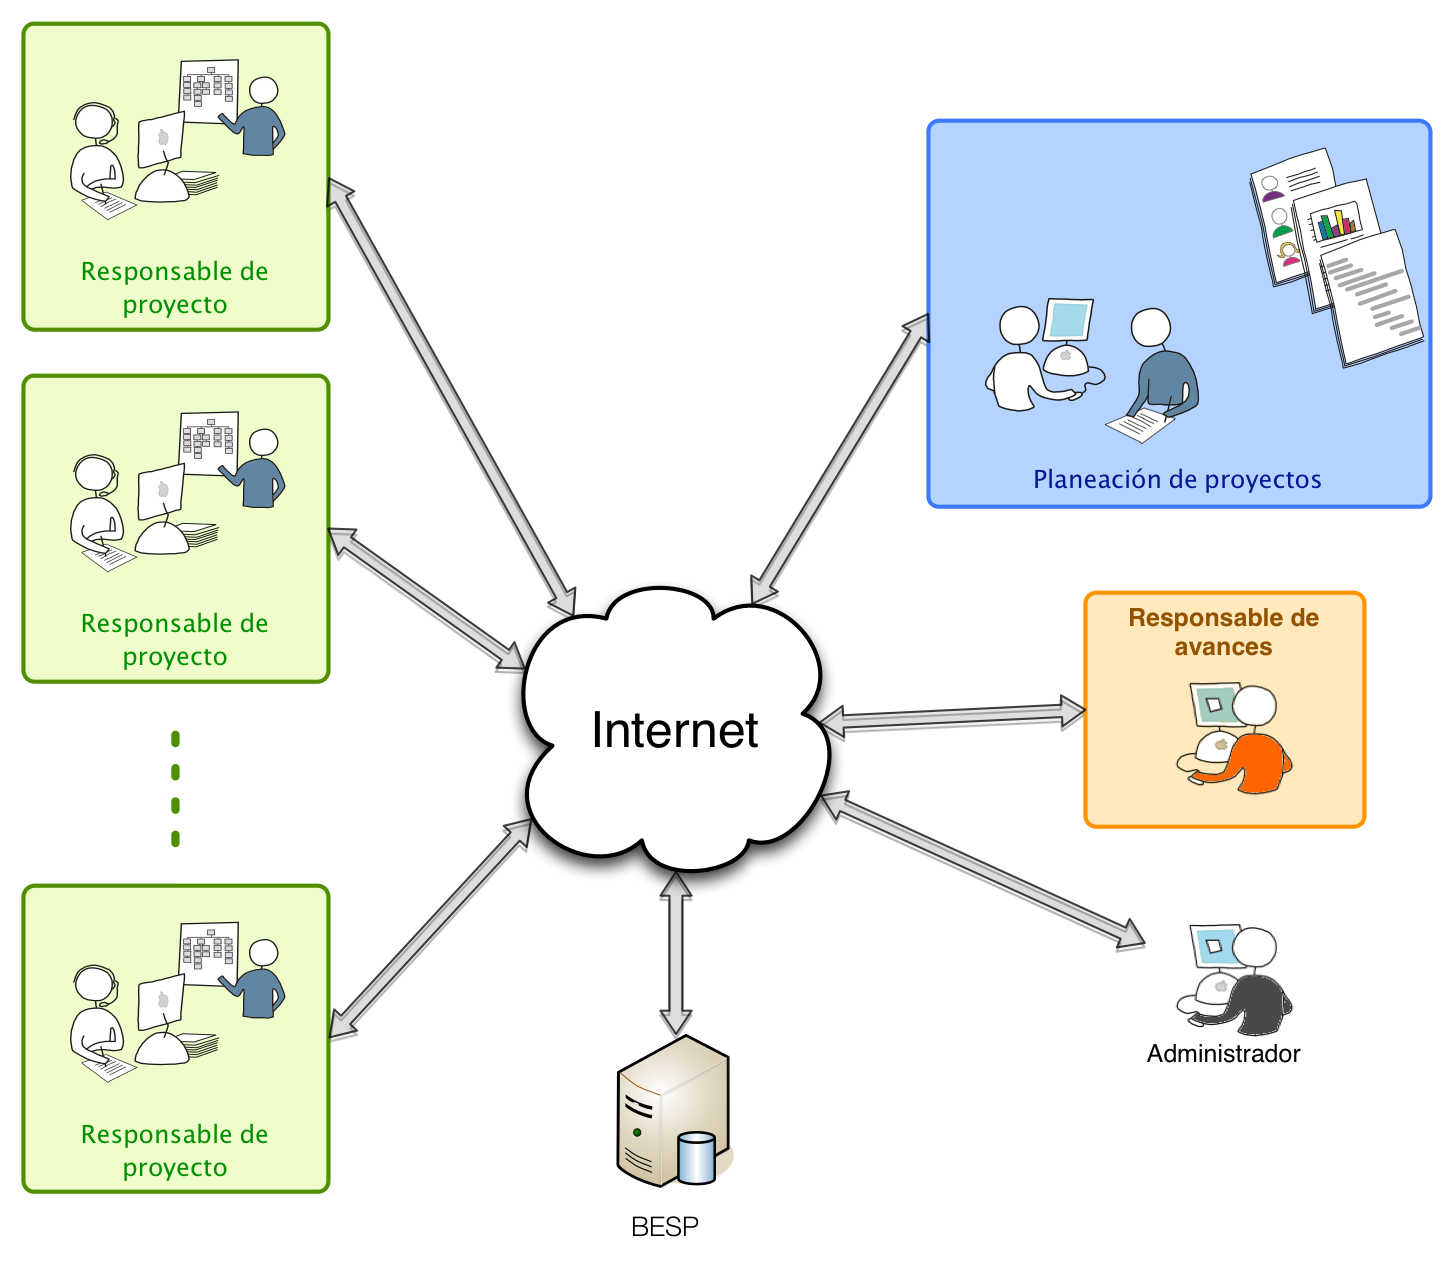
\includegraphics[width=.6\textwidth]{images/arquitectura}}
		\caption{Arquitectura del sistema.}
		\label{fig:arquitectura}
	\end{center}
\end{figure}

En la figura~\ref{fig:arquitectura} se describe la estructura del sistema, en ella se detalla ...


%---------------------------------------------------------
\section{Diseño de interfaces}

\cdtInstrucciones{
	Indique el tipo de interfaces que deberá tener el sistema: consola, móviles, texto, audio, WEB, de escritorio, etc.\\
	
	Presente un mapa de navegación entre pantallas y describa cada una de las pantallas.
	
	Para cada pantalla o interfaz describa:
	
\begin{description}
	\item[Id de la pantalla:] IUX
	\item[Nombre:] Nombre de la pantalla.
	\item[Diseño de la pantalla:] Dibujo o bosquejo de la pantalla.
	\item[Descripción de uso:] Al menos un párrafo que describa como se debe usar la pantalla o interfaz.
\end{description}
}

% - - - - - - - - - - - - - - - - - - - - - - - - - - - - - 
\subsection{Modelo de navegación}

	La navegación entre pantallas se muestra en la figura~\ref{fig:mapa}. en el se explica ...\\

\begin{figure}[htbp]
	\begin{center}
		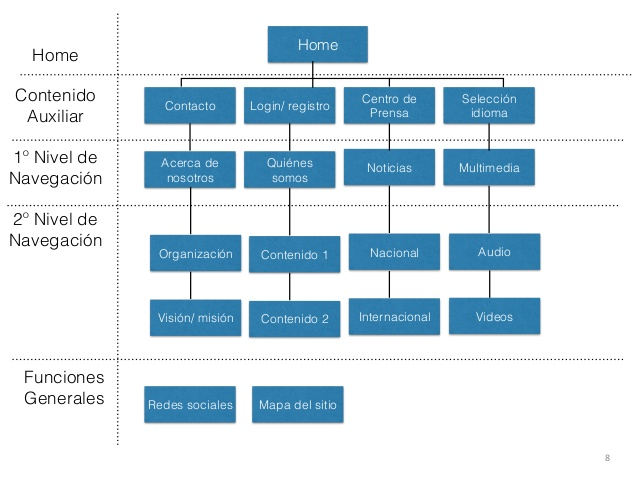
\includegraphics[width=.7\textwidth]{images/mapa}
		\caption{mapa}
		\label{fig:mapa}
	\end{center}
\end{figure}

% - - - - - - - - - - - - - - - - - - - - - - - - - - - - - 
\subsection{IU23 Pantalla de Control de Acceso}

\subsubsection{Objetivo}
	Controlar el acceso al sistema mediante una contraseña a fin de que cada usuario acceda solo a las operaciones permitidas para su perfil.

\subsubsection{Diseño}
	Esta pantalla \IUref{IU23}{Pantalla de Control de Acceso} (ver figura~\ref{IU23}) aparece al iniciar el sistema. Para ingresar al mismo se debe escribir el Número de Boleta del estudiante y la contraseña de acceso. 

\IUfig[.5]{Login}{IU23}{Pantalla de Control de Acceso.}

\subsubsection{Salidas}

	Ninguna.

\subsubsection{Entradas}
Número de Boleta y Contraseña del Estudiante.

\subsubsection{Comandos}
\begin{itemize}
	\item \IUbutton{Entrar}: Verifica que el Estudiante se encuentre registrado y la contraseña sea la correcta. Si la verificación es correcta, se muestra la \IUref{UI32}{Pantalla de Selección de Seminario}.
	\item \IUbutton{Ayuda}: Muestra la ayuda de esta pantalla \IUref{IU50}{Pantalla de Ayuda}.
\end{itemize}

\subsubsection{Mensajes}

\begin{Citemize}
	\item Error al verificar los datos de acceso, vuelva a intentarlo.
\end{Citemize}



